% Musharraf's CV in LaTeX

\documentclass[10pt,a4paper]{article}

\usepackage[margin=0.7in]{geometry}
\usepackage[T1]{fontenc}
\usepackage[utf8]{inputenc}
\usepackage{lmodern}
\usepackage{microtype}
\usepackage{enumitem}
\usepackage{titlesec}
\usepackage{xcolor}
\usepackage[hidelinks]{hyperref}
\usepackage{fontawesome5}
\usepackage{graphicx}

\pagestyle{empty}
\setlength{\parindent}{0pt}
\definecolor{accent}{HTML}{1F3A5F}

% Section headings
\titleformat{\section}{\large\bfseries\color{accent}}{}{0em}{}[\titlerule]
\titlespacing{\section}{0pt}{10pt}{5pt}

% Compact bullet lists
\setlist[itemize]{leftmargin=1.2em, itemsep=1pt, topsep=2pt, parsep=0pt}

% \cventry{Title}{Date}{Organisation}{Location}
\newcommand{\cventry}[4]{%
  \textbf{#1} \hfill #2\\
  \textit{#3} \hfill \textit{#4}\vspace{1pt}}

% \project{Name}{Tech stack}{Date}
\newcommand{\project}[3]{%
  \textbf{#1} $|$ \textit{#2} \hfill #3}

\begin{document}

%---------------- HEADER ----------------
\noindent
\begin{minipage}[c]{0.22\textwidth}
  \centering
  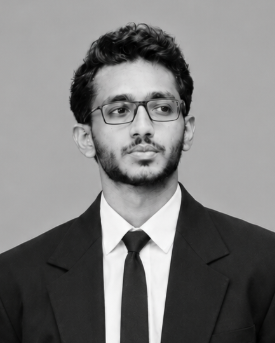
\includegraphics[width=1.0\linewidth, height=4cm,width=3.2cm]{Me_Black.png}
\end{minipage}%
\hfill
\begin{minipage}[c]{0.78\textwidth}
  \centering
  {\LARGE\bfseries Mohamed Rauf Abdur Rahman Musharraf}\\[5pt]
  \vspace{10pt}
  \faPhone \hspace{0.1cm} +94 77 5451054 \;$|$
  \faEnvelope \href{mailto:musharrafcm97@outlook.com}{ musharrafcm97@outlook.com} \; $|$ \faGithub \href{https://github.com/musharraf-mac}{ Musharraf-mac} \\
  \faLinkedin \href{https://www.linkedin.com/in/abdur-rahman-musharraf/}{ /in/abdur-rahman-musharraf} \; $|$ \faGlobe \href{https://armusharraf.me}{ armusharraf.me} $|$
  \faMapMarker* Colombo, Sri Lanka \\
  \vspace{2pt}
  \faLanguage \hspace{0.1cm}Tamil(Native) $|$ English(Intermediate) $|$ Sinhala(basic)
\end{minipage}

%---------------- SUMMARY ----------------
\section{Summary}
Results-driven IT undergraduate with a strong foundation in Python, SQL, database management, data preprocessing, and software engineering. Experienced in working with structured and unstructured data, performing data cleaning, transformation, and analysis using Python, Pandas, and NumPy. Familiar with relational and NoSQL databases, including PostgreSQL, MySQL, and MongoDB, alongside cloud platforms such as Google Cloud, AWS, and Azure. Experienced in REST API development, AI-assisted coding tools, and machine learning projects. Brings strong analytical thinking, problem-solving abilities, and attention to detail. Eager to develop scalable data pipelines, explore modern data engineering technologies, and contribute to enterprise-scale data solutions within a collaborative environment.

%---------------- EDUCATION ----------------
\section{Education}
\begin{itemize}[itemsep=8pt]
\item \cventry{BSc (Hons) in Information Technology}{2024 -- Present}{Horizon Campus}{Malabe, Sri Lanka}
\item \cventry{Diploma in Software Engineering}{2023 -- 2025}{Wayamba University of Sri Lanka}{Kuliyapitiya, Sri Lanka}
\item \cventry{GCE (A/L) - Physical Science Stream}{2018 -- 2021}{BT/BC/Al-Hira Maha Vidyalaya}{Kattankudy. Sri Lanka}

\end{itemize}
%---------------- PROJECTS ----------------
\section{Projects}

\begin{enumerate}
  % Project - 1
  \item \project{Multimodal Explainable AI for Tuberculosis Diagnosis}{AI model \& research Tool - Pair work}{2026}
   \begin{itemize}
    \item Developed a research prototype combining DenseNet-based chest X-ray analysis with Grad-CAM visual explanations. Integrated a symptom-text analysis component and SHAP-based explanations to support model interpretability
    \item \textbf{Applied Technologies}: Python, Pytorch, Deep learning, Densnet, Jupyter notebook, Pandas, SHAP, GradCam, NLP
    \item \faGithub \href{https://github.com/musharraf-Mac/Detective-XAI-For-TB}{ musharraf-Mac/Detective-XAI-For-TB} \hspace{0.15cm} $|$ \hspace{0.15cm} \faLink \href{https://detective-xai-for-tb.streamlit.app}{ detective-xai-for-tb.streamlit.app}
   \end{itemize}


  % Project - 2
  \item \project{Literature review Agent}{Agentic AI}{2023}
   \begin{itemize}
    \item An agentic AI application that automates literature review generation for a given research topic — searching academic sources, filtering and embedding relevant papers, formulating research sub-questions, retrieving grounded answers via RAG, and synthesizing a coherent literature review
    \item \textbf{Applied Technologies}: Langchain, Python, RAG, LLM APIs
    \item \faGithub \href{https://github.com/musharraf-Mac/Literature-review-agentic-AI}{ musharraf-Mac/Literature-review-agentic-AI} \hspace{0.2cm} $|$ \hspace{0.2cm} \faLink \href{https://literature-review-agentic-ai.streamlit.app/}{ literature-review-agentic-ai.streamlit.app}
   \end{itemize}
  

   % Project - 3
  \item \project{Health System}{Microservice Web system - Group project}{2026}
   \begin{itemize}
    \item Health web system used for book doctor and treat a patient and update it to the patient profile. Also, public can calculate their BMI and if user logged in it will save it inside history also lab report will be analyzed by AI and give a brief to the user
    \item \textbf{Applied Technologies}: NextJs, Tailwindcss, Typescript, Springboot, mongoDB, JWT,Redis, Docker
    \item \textbf{Deployed in:}
      \begin{itemize}
        \item \textbf{Front-end:} netlify
        \item \textbf{Back-end:} GCP - Cloud run
        \item \textbf{DataBase:} MongoDB Atlas
      \end{itemize}
    \item My role: Leader \& Full Stack developer
    \item \faGithub \href{https://github.com/musharraf-Mac/SOC-AI-Health-Web-System}{ musharraf-Mac/SOC-AI-Health-Web-System} \hspace{0.15cm} $|$ \hspace{0.15cm} \faLink \href{https://health-web-system.netlify.app/}{ health-web-system.netlify.app/}
   \end{itemize}

\end{enumerate}
\vspace{8pt}
\section{Projects - Continued}

\begin{enumerate}[resume]
   % Project - 4
  \item \project{AI - Text detector}{AI model - Group Project}{2026}
  \begin{itemize}
    \item Collaborated in a five-member team to build a text classifier using TF-IDF and logistic regression. The baseline achieved 94% accuracy on an imbalanced test set, and the team evaluated false positives and performance on paraphrased text and text from an unseen AI generator
    \item \textbf{Applied Technologies: }Python, Pandas, numpy, scikit-learn, TF-IDF, Matplotlib, Seaborn, Jupyter notebook, Streamlit, pickle
    \item \textbf{My role: }Leader, Trained the model, Data preparation, Data Collection
  \end{itemize}

   % Project - 5
   \item \project{Lankan Tourism Website}{Website}{2026}
   \begin{itemize}
    \item Built a website for a tourism agency named as Lankan tourism
    \item In here you can view their services and can see the review of the past customers and can add your review if you were one of the customers
    \item And the services and whatsapp button will redirect you to their official whatsapp number
    \item \textbf{Applied Technologies}: NextJS, Typescript, Tailwindcss, Firestore, GCP
    \item \faLink \href{https://lankantourism.lk}{ www.lankantourism.lk}
   \end{itemize}
   % Project - 6

\end{enumerate}
\begin{itemize}
  \item \textbf{Check my \href{https://armusharraf.me}{\textcolor{accent}{website}} \& \href{https://github.com/musharraf-Mac}{\textcolor{accent}{Github}} for more projects}
\end{itemize}

%---------------- EXPERIENCE ----------------
\section{Experience}
\cventry{Free lancer}{2022 - present}{My Self}{Sri Lanka}
\begin{itemize}
  \item Web Development project : Developed a Tourism website : www.lankantourism.lk
  \item Other projects - Prepares documents such as books \& exam papers using microsoft applications
\end{itemize}

%---------------- SKILLS ----------------
\section{Technical Skills}
\begin{itemize}[leftmargin=2pt, label={}, itemsep=2pt]
  \item \textbf{Programming Languages:} c\#(.net), Java, C, Python, Typescript, JavaScript
  \item \textbf{Data Engineering: }Apache PySpark, Data Preprocessing, Data transformation
  \item \textbf{Data Analytics \& Visualization: }Pandas, Numpy, Power BI, Matplotlib, Seaborn
  \item \textbf{Databases:} MongoDB, MySQL, PostgreSQL, Firestore
  \item \textbf{DeVop tools:} Git, GitHub, Docker, Kubernetes, CI/CD
  \item \textbf{Deployment \& Cloud:} GCP, AWS, Azure, Vercel, Render, Infinitefree, Supabase, Cloudinary, Netlify
  \item \textbf{Front-End:} ReactJS, Typescript, JavaScript, CSS, TailwindCSS, HTML, NextJS, Angular
  \item \textbf{Back-End:} Spring-boot(Java), Laravel(PHP), ExpressJS(NodeJS), FastAPI, Django(Python)
  \item \textbf{Mobile app Development:} Kotlin, Java, XML, Android Studio, React Native
  \item \textbf{Machine Learning / AI:} Pytorch, Python, Langchain, Agentic AI, Scikit-learn, RAG
  \item \textbf{Design: }Figma, Canva
  \item \textbf{AI-Assist development } Codex, Continue, Github Copilot, Claude code, Antigravity
  
\end{itemize}

%---------------- ACHIEVEMENTS ----------------
\section{Extra Carricular Activities}
\begin{itemize}
  \item Executive board member of Student council \& Sports council
  \item Member of the Leo Club, Chess Club, E-sports Club, and Cyber Security Community at Horizon Campus.
  \item Participated in chess tournaments in Campus
  \item Participated in marathon organized by Management faculty in horizon campus.
\end{itemize}

\section{Certifications}
 \begin{itemize}
  \item Python for Beginners by University of Moratuwa
  \item AI/ML Engineer By SLIIT
  \item Intro to programming -- Kaggle
 \end{itemize}

\section{References}
\begin{minipage}[t]{0.3\textwidth}
\textbf{Mr. Anjana Abeykoon} \\
Senior Lecturer \\
Faculty of IT \\
Horizon Campus. \\
anjana@horizoncampus.edu.lk
\end{minipage}
\hfill
\begin{minipage}[t]{0.3\textwidth}
  \textbf{Mr. Isuru Samarappulige} \\
  Senior Lecturer \\
  Faculty of IT \\
  Horizon Campus \\
  Isuru@horizoncampus.edu.lk \\
\end{minipage}
\hfill
\begin{minipage}[t]{0.3\textwidth}
  \textbf{Mr.Sankha Wijayawardhana} \\
  Senior Lecturer \\
  Faculty of IT \\
  Horizon Campus \\
  sankha@horizoncampus.edu.lk
\end{minipage}
\end{document}